% 92-20(92쪽) — 한 직선 위의 세 점 B, C, D 와 그 위의 두 점 A, E(원문 「오른쪽 그림」). 스캔 화질이 낮아 TikZ 로 다시 그림.
% 라벨은 원문 것만: 꼭짓점 A·B·C·D·E, 길이 3·5, 30° 두 개, 직각 표시 두 개.
% 선분 AE 의 길이(답)는 그림에 적지 않는다.
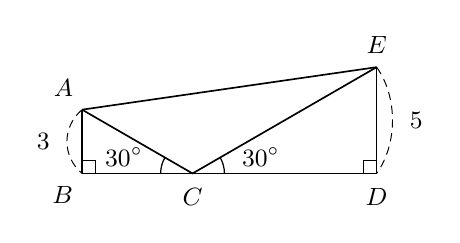
\begin{tikzpicture}[line width=0.6pt, x=0.27cm, y=0.27cm]
  \coordinate (A) at (0,3);
  \coordinate (B) at (0,0);
  \coordinate (C) at (5.196,0);
  \coordinate (D) at (13.856,0);
  \coordinate (E) at (13.856,5);
  \draw (B) -- (D);
  \draw (A) -- (B);
  \draw (E) -- (D);
  \draw (A) -- (E);
  \draw (A) -- (C) -- (E);
  % 직각 표시
  \draw[line width=0.45pt] (0.62,0) -- (0.62,0.62) -- (0,0.62);
  \draw[line width=0.45pt] (13.236,0) -- (13.236,0.62) -- (13.856,0.62);
  % 30° 각 표시
  \draw[line width=0.45pt] ([shift={(150:1.5)}]C) arc [start angle=150, end angle=180, radius=1.5];
  \draw[line width=0.45pt] ([shift={(0:1.5)}]C) arc [start angle=0, end angle=30, radius=1.5];
  % 길이 표시의 점선 호
  \draw[densely dashed, line width=0.35pt] (A) .. controls (-0.95,2.2) and (-0.95,0.8) .. (B);
  \draw[densely dashed, line width=0.35pt] (E) .. controls (14.85,3.6) and (14.85,1.4) .. (D);
  \node[font=\small, anchor=south east] at (0.05,3.15) {$\pt{A}$};
  \node[font=\small, anchor=north east] at (0.05,-0.15) {$\pt{B}$};
  \node[font=\small, anchor=north] at (5.196,-0.25) {$\pt{C}$};
  \node[font=\small, anchor=north] at (13.856,-0.25) {$\pt{D}$};
  \node[font=\small, anchor=south] at (13.856,5.15) {$\pt{E}$};
  \node[font=\small, anchor=east] at (-1.05,1.5) {$3$};
  \node[font=\small, anchor=west] at (14.95,2.5) {$5$};
  \node[font=\small] at (1.97,0.78) {$30^\circ$};
  \node[font=\small] at (8.41,0.78) {$30^\circ$};
\end{tikzpicture}
